The Large Hadron Collider (LHC) \cite{LHCTDR} is a duel-ring high-energy particle accelerator and collider located at CERN, the European Laboratory for Particle Physics, in Geneva, Switzerland. Built in the tunnel of the dismantled LEP collider $\SI{50}{m}$ below the Swiss-French border (see Fig.~\ref{fig:LHC}), the LHC spans $\SI{27}{km}$ in circumference and currently holds the world record for the highest-energy particle collisions at a center-of-mass energy $\sqrt{s} = \SI{13}{TeV}$. Four independent detectors located at points along the circumference of the LHC record the collisions: Compact Muon Solenoid (CMS), A Toroidal LHC ApparatuS (ATLAS), Large Hadron Collider beauty (LHCb), and A Lead Ion Collider Experiment (ALICE).

\begin{figure}[H]
    \centering
    \resizebox{1\textwidth}{!}{
    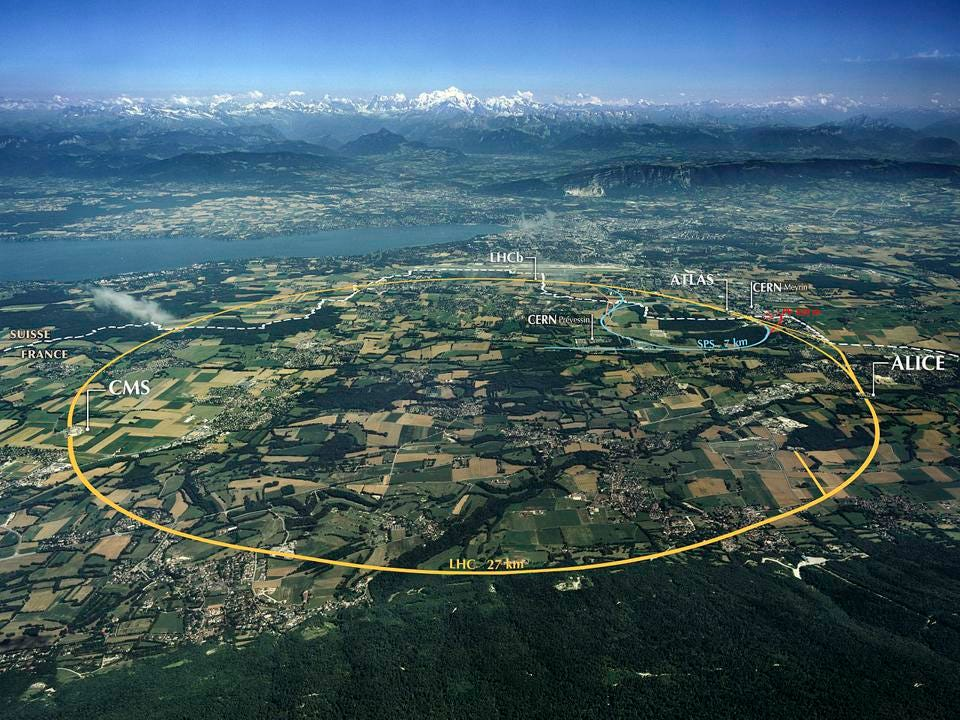
\includegraphics[height=\textwidth]{Images/CMS/LHCring.jpg}
    \quad
    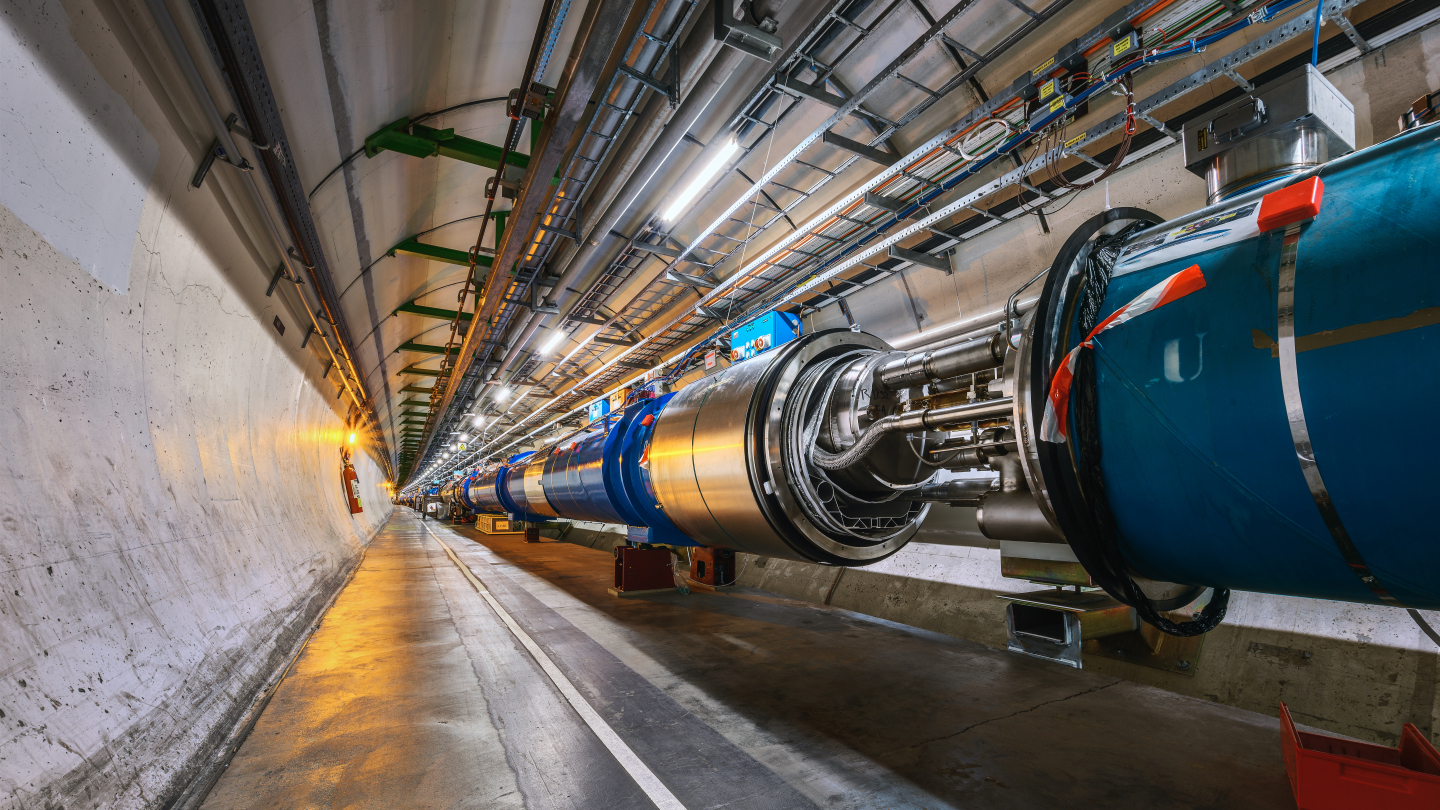
\includegraphics[height=\textwidth]{Images/CMS/LHCpipe.jpg}
    }
    \caption{Left: A tracing of the LHC tunnel over the Swiss-French border near Geneva. Right: A section of the LHC beam pipe in the underground LHC tunnel.}
    \label{fig:LHC}
\end{figure}

Within the LHC, two beams of protons or heavy ions are accelerated in opposite directions, captured and stored by $\SI{400}{MHz}$ radiofrequency (RF) cavities located at 16 points along the LHC ring that longitudinally sort the beams into 2808 bunches of $\SI{1.15e11}{}$ protons or Pb ions, with each bunch spaced $\SI{25}{ns}$ apart. The beams at the LHC are steered along each ring by 1232 $\SI{8.3}{T}$ superconducting dipole magnets, while 392 superconducting quadrupole magnets focus the beams into a narrow transverse cross section of $\SI{3.8}{\micro\meter}$. The beams cross at four insertion points along the LHC, where the proton-proton or lead ion collisions occur and are recorded by each of the four LHC experiments.

The LHC was designed to operate in several sequencial phases. Phase-1 saw first collisions at $\sqrt{s}=\SI{7}{TeV}$ in 2010 which was increased to $\sqrt{s}=\SI{13}{TeV}$ in 2015. Phase-2 of the LHC will raise the instantanious luminosity by a factor of ten, called the High-Luminosity LHC (HL-LHC) era, slated to begin operation in 2027. Upgrades to the LHC and detectors are performed during long shutdown (LS) periods that separate data-taking runs.

The physics goals of the LHC could be broadly summerized with the following: to observe the last undiscovered particle in the SM, the Higgs boson; to search for evidence of beyond the SM physics; and to perform precision measurements of existing SM phenomena. On July 4th, 2012 it was announced that the ATLAS and CMS collaborations had independently observed the Higgs boson, which remains the hallmark achievement at the LHC.